%%%%%%%%%%%%%%%%%%%%%%%%%%%%%%%%%%%%%%%%%%%%%%%%%%%%%%%%%%%%%%%%%%%%%%%%%%%%%%%%
%                            Document Information                              %
% ---------------------------------------------------------------------------- %
% Document Title: Math Behind Popular Trading Indicators                       %
% Date Created: 2025/01/06                                                     %
% Version: 1.2.0                                                               %
% ---------------------------------------------------------------------------- %
% Purpose: Highlighting the critical role of mathematics in trading.           %
% ---------------------------------------------------------------------------- %
% Last Updated: 2025/01/09                                                     %
%%%%%%%%%%%%%%%%%%%%%%%%%%%%%%%%%%%%%%%%%%%%%%%%%%%%%%%%%%%%%%%%%%%%%%%%%%%%%%%%

% TODO List:
% - Update Abstract
% - Indicators needed to add:
%   - Trend Indicators (SMA, EMA, MACD, ADX)
%   - Momentum Indicators (RSI, Stochastic Oscillator, CCI, ROC)
%   - Volatility Indicators (Bollinger Bands, ATR)
%   - Volume Indicators (OBV, MFI, VWAP)
%   - Additional Indicators (Ichimoku Cloud)

%%%%%%%%%%%%%%%%%%%%%%%%%%%%%%%%%%%%%%%%%%%%%%%%%%%%%%%%%%%%%%%%%%%%%%%%%%%%%%%%
%                         Preamble Setup for Document                          %
%%%%%%%%%%%%%%%%%%%%%%%%%%%%%%%%%%%%%%%%%%%%%%%%%%%%%%%%%%%%%%%%%%%%%%%%%%%%%%%%

% --- General Document Settings ------------------------------------------------
\documentclass[12pt]{article}

% --- Page Layout and Geometry -------------------------------------------------
\usepackage[letterpaper, margin=1in]{geometry}

% --- Font and Microtype Settings ----------------------------------------------
\usepackage{microtype}

% --- Mathematical Symbols and Fonts -------------------------------------------
\usepackage{amsmath}
\usepackage{amssymb}
\usepackage{amsthm}
\usepackage{amsfonts}
\usepackage{mathrsfs}
\usepackage{bm}
\usepackage{mathtools}

% --- Tables and Arrays --------------------------------------------------------
\usepackage{booktabs}
\usepackage{makecell}
\usepackage{tabularray}

% --- Graphics and Color -------------------------------------------------------
\usepackage{graphicx}
\usepackage{xcolor}
\usepackage{pgfplots}

% --- Section and Formatting Control -------------------------------------------
\usepackage{titlesec}
\usepackage{setspace}
\usepackage{parskip}
\usepackage{ragged2e}
\usepackage{lipsum}
\usepackage{epigraph}
\usepackage{titletoc}

% --- Text Formatting ----------------------------------------------------------
\usepackage[normalem]{ulem}
\usepackage{mdframed}
\usepackage{hyphenat}

% --- Lists and Enumerations ---------------------------------------------------
\usepackage{enumitem}

% --- Hyperlinks and URLs ------------------------------------------------------
\usepackage{url}
\usepackage{hyperref}

% --- Miscellaneous ------------------------------------------------------------
\usepackage{circledsteps}
\usepackage{fancyhdr}

% \usepackage{tikz}
% \usetikzlibrary{patterns}
% \usetikzlibrary{backgrounds}

%%%%%%%%%%%%%%%%%%%%%%%%%%%%%%%%%%%%%%%%%%%%%%%%%%%%%%%%%%%%%%%%%%%%%%%%%%%%%%%%
%                       Custom Commands and Environments                       %
%%%%%%%%%%%%%%%%%%%%%%%%%%%%%%%%%%%%%%%%%%%%%%%%%%%%%%%%%%%%%%%%%%%%%%%%%%%%%%%%

% --- Theorem Environments Formatting ------------------------------------------
\theoremstyle{plain}
\newtheorem*{definition}{Definition}

% --- Table of Contents Depth --------------------------------------------------
\setcounter{tocdepth}{2}

% --- Page Layout and Geometry -------------------------------------------------
\geometry{
  top=2.2cm,
  headheight=0mm,
  headsep=0mm,
}
\pagestyle{fancy}
\fancyhf{}

% --- Header and Footer Rules --------------------------------------------------
\renewcommand{\headrulewidth}{0pt}
\renewcommand{\footrulewidth}{0pt}
\setlength{\footskip}{44pt}
\fancyfoot[C]{\thepage}

% --- Section Formatting -------------------------------------------------------
\titleformat{\section}
{\Huge\bfseries}
{}
{0pt}
{}

% --- Spacing Definitions ------------------------------------------------------
\pgfplotsset{compat=newest}

% --- Title Page Decoration ----------------------------------------------------
\renewcommand\epigraphflush{flushright}
\renewcommand\epigraphsize{\normalsize}
\setlength\epigraphwidth{0.7\textwidth}

\definecolor{titlepagecolor}{cmyk}{0,0,0,1}

\DeclareFixedFont{\titlefont}{T1}{ppl}{b}{it}{0.5in}

\makeatletter                       
\def\printauthor{%                  
    {\large \@author}}              
\makeatother

\newcommand\titlepagedecoration{%
\begin{tikzpicture}[remember picture,overlay,shorten >= -10pt]

\coordinate (aux1) at ([yshift=-15pt]current page.north east);
\coordinate (aux2) at ([yshift=-410pt]current page.north east);
\coordinate (aux3) at ([xshift=-4.5cm]current page.north east);
\coordinate (aux4) at ([yshift=-150pt]current page.north east);

\begin{scope}[titlepagecolor!60,line width=14pt,rounded corners=16pt] % Changed color and line width
\draw
  (aux1) -- coordinate (a)
  ++(225:5) -- 
  ++(-45:5.1) coordinate (b);
\draw[shorten <= -10pt]
  (aux3) --
  (a) --
  (aux1);
\draw[opacity=0.7,titlepagecolor,shorten <= -10pt] % Increased opacity
  (b) -- 
  ++(225:2.4) -- 
  ++(-45:2.4);
\end{scope}
\draw[titlepagecolor,line width=10pt,rounded corners=10pt,shorten <= -10pt] % Increased line width
  (aux4) --
  ++(225:0.9) --
  ++(-45:0.9);
\begin{scope}[titlepagecolor!80,line width=8pt,rounded corners=10pt] % Changed color and line width
\draw[shorten <= -10pt]
  (aux2) --
  ++(225:3.2) coordinate[pos=0.45] (c) --
  ++(-45:3.2);
\draw
  (aux2) --
  (c) --
  ++(135:2.6) -- 
  ++(45:2.6) -- 
  ++(-45:2.6) coordinate[pos=0.3] (d);   
\draw 
  (d) -- +(45:1.2);
\end{scope}
\end{tikzpicture}%
}

% --- Table of Contents Formatting --------------------------------------------
\titlecontents{section}[2.3em]
  {}
  {\bfseries\contentslabel[\thecontentslabel.0]{2em}\MakeUppercase}
  {\hspace*{-2.3em}\bfseries\MakeUppercase}
  {\titlerule*[1pc]{.}\contentspage}
\titlecontents{subsection}[4.6em]
  {}
  {\bfseries\contentslabel{2em}}
  {\hspace*{-2.3em}\bfseries}
  {\titlerule*[1pc]{.}\contentspage}
\titlecontents{subsubsection}[6.9em]
  {}
  {\bfseries\contentslabel{2em}\itshape\space}
  {\hspace*{-2.3em}\bfseries}
  {\titlerule*[1pc]{.}\contentspage}

\makeatletter
\renewcommand\tableofcontents{%
  \section*{\centerline{\MakeUppercase{\contentsname}}
    \@mkboth
      {\MakeUppercase\contentsname}
      {\MakeUppercase\contentsname}
  }%
  \@starttoc{toc}%
}
\makeatother

%%%%%%%%%%%%%%%%%%%%%%%%%%%%%%%%%%%%%%%%%%%%%%%%%%%%%%%%%%%%%%%%%%%%%%%%%%%%%%%%
%                            End of Preamble Setup                             %
%%%%%%%%%%%%%%%%%%%%%%%%%%%%%%%%%%%%%%%%%%%%%%%%%%%%%%%%%%%%%%%%%%%%%%%%%%%%%%%%

\begin{document}

%%%%%%%%%%%%%%%%%%%%%%%%%%%%%%%%%%%%%%%%%%%%%%%%%%%%%%%%%%%%%%%%%%%%%%%%%%%%%%%%
%                                Title Page                                    %
%%%%%%%%%%%%%%%%%%%%%%%%%%%%%%%%%%%%%%%%%%%%%%%%%%%%%%%%%%%%%%%%%%%%%%%%%%%%%%%%
\begin{titlepage}

\noindent
\titlefont Math Behind Popular \\ Trading Indicators\par

\vspace{0.7cm}

\begin{quote}
    \textit{All the math you need in the stock market you get in the fourth grade.}
\end{quote}

\begin{center}
  \textsc{\hspace{-1.4cm}-- Peter Lynch --}
\end{center}

\vspace{2.5cm}

\begin{figure}[h]
    \centering
    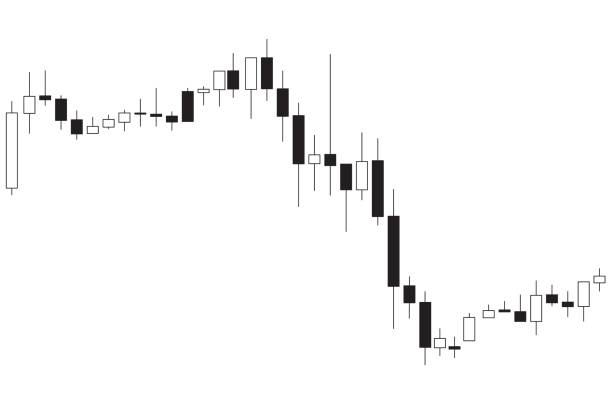
\includegraphics[width=0.75\textwidth]{../images/chart.jpg}
\end{figure}

\vfill

\begin{center}
    \textsc{\large PRIME BEHOOF}
\end{center}

\titlepagedecoration
\end{titlepage}


%%%%%%%%%%%%%%%%%%%%%%%%%%%%%%%%%%%%%%%%%%%%%%%%%%%%%%%%%%%%%%%%%%%%%%%%%%%%%%%%
%                                End Title Page                                %
%%%%%%%%%%%%%%%%%%%%%%%%%%%%%%%%%%%%%%%%%%%%%%%%%%%%%%%%%%%%%%%%%%%%%%%%%%%%%%%%

\newpage

%%%%%%%%%%%%%%%%%%%%%%%%%%%%%%%%%%%%%%%%%%%%%%%%%%%%%%%%%%%%%%%%%%%%%%%%%%%%%%%%
%                           Begin Table of Contents                            %
%%%%%%%%%%%%%%%%%%%%%%%%%%%%%%%%%%%%%%%%%%%%%%%%%%%%%%%%%%%%%%%%%%%%%%%%%%%%%%%%

\tableofcontents

%%%%%%%%%%%%%%%%%%%%%%%%%%%%%%%%%%%%%%%%%%%%%%%%%%%%%%%%%%%%%%%%%%%%%%%%%%%%%%%%
%                            End Table of Contents                             %
%%%%%%%%%%%%%%%%%%%%%%%%%%%%%%%%%%%%%%%%%%%%%%%%%%%%%%%%%%%%%%%%%%%%%%%%%%%%%%%%

\newpage

%%%%%%%%%%%%%%%%%%%%%%%%%%%%%%%%%%%%%%%%%%%%%%%%%%%%%%%%%%%%%%%%%%%%%%%%%%%%%%%%
%                               Begin Abstract                                 %
%%%%%%%%%%%%%%%%%%%%%%%%%%%%%%%%%%%%%%%%%%%%%%%%%%%%%%%%%%%%%%%%%%%%%%%%%%%%%%%%

\begin{abstract}
  Need to update.
\end{abstract}

%%%%%%%%%%%%%%%%%%%%%%%%%%%%%%%%%%%%%%%%%%%%%%%%%%%%%%%%%%%%%%%%%%%%%%%%%%%%%%%%
%                                End Abstract                                  %
%%%%%%%%%%%%%%%%%%%%%%%%%%%%%%%%%%%%%%%%%%%%%%%%%%%%%%%%%%%%%%%%%%%%%%%%%%%%%%%%

\newpage

%%%%%%%%%%%%%%%%%%%%%%%%%%%%%%%%%%%%%%%%%%%%%%%%%%%%%%%%%%%%%%%%%%%%%%%%%%%%%%%%
%                          Begin Section: Disclaimers                          %
%%%%%%%%%%%%%%%%%%%%%%%%%%%%%%%%%%%%%%%%%%%%%%%%%%%%%%%%%%%%%%%%%%%%%%%%%%%%%%%%

\section{DISCLAIMERS}

In the discussion below, I will adopt the following conventions:  

\begin{itemize}
  \item Price data points may correspond to one of the following values:  
    \begin{itemize}
      \item $O$: Open  
      \item $H$: High  
      \item $L$: Low  
      \item $C$: Close  
    \end{itemize}
  \item Unless explicitly specified, $P$ will serve as a placeholder for any of these price data points.
  \item Let $P$ represent a price value. The observed price at time $t$ is denoted as $P_t$, the price of the previous candle as $P_{t-1}$, and the price of the next candle as $P_{t+1}$.
  \item If not explicity specified, standard lookback period will have length of $n$.
\end{itemize}

\begin{center}
  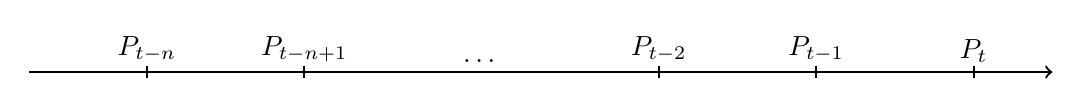
\begin{tikzpicture}[scale=1]
    % ------------------------------------------------------------------------ %
    % Plot-Name: Indexing Line Explanation Plot                                %
    % ------------------------------------------------------------------------ %

    % Horizontal line
    \draw[thick, ->] (0,0) -- (13,0);

    % Ticks on line
    \foreach \x in {1.5, 3.5, 8, 10, 12} {
        \draw[thick] (\x,0.08) -- (\x,-0.08);
    }

    % Ticks labels
    \node[above] at (1.5,0) {$P_{t-n}$};
    \node[above] at (3.5,0) {$P_{t-n + 1}$};
    \node[above] at (5.75,0) {\ldots};
    \node[above] at (8,0) {$P_{t-2}$};
    \node[above] at (10,0) {$P_{t-1}$};
    \node[above] at (12,0) {$P_t$};

  \end{tikzpicture}
\end{center}

Now that we have clarified the conventions of notation and indexing system, let us proceed with the discussion of indicators.

%%%%%%%%%%%%%%%%%%%%%%%%%%%%%%%%%%%%%%%%%%%%%%%%%%%%%%%%%%%%%%%%%%%%%%%%%%%%%%%%
%                           End Section: Disclaimers                           %
%%%%%%%%%%%%%%%%%%%%%%%%%%%%%%%%%%%%%%%%%%%%%%%%%%%%%%%%%%%%%%%%%%%%%%%%%%%%%%%%

\newpage

%%%%%%%%%%%%%%%%%%%%%%%%%%%%%%%%%%%%%%%%%%%%%%%%%%%%%%%%%%%%%%%%%%%%%%%%%%%%%%%%
%                         Begin Section: Trend Indicators                      %
%%%%%%%%%%%%%%%%%%%%%%%%%%%%%%%%%%%%%%%%%%%%%%%%%%%%%%%%%%%%%%%%%%%%%%%%%%%%%%%%

\section{TREND INDICATORS}

\begin{definition} \textbf{Simple Moving Average - SMA} \\
Tool in financial analysis that computes the arithmetic mean of a security's price over a predetermined number of periods. By averaging past prices, the SMA smooths out price fluctuations, aiding in the identification of prevailing market trends.
\end{definition}

\vspace{-15pt}

$$ S\!M\!A_t(n) \, = \, \sum_{k = 0}^{n-1} \, P_{t - k} $$

\begin{definition} \textbf{Exponential Moving Average - EMA} \\
Weighted moving average that places greater importance on recent price data. The EMA is calculated by applying a smoothing factor to the previous period's EMA and the current period's price.
\end{definition}

\vspace{-10pt}

$$ 
E\!M\!A_t(n) \, = \, \alpha \cdot P_t \, + \, (1 - \alpha) \cdot E\!M\!A_{t-1}(n)
$$

\textit{It offers a more responsive average, reflecting current market trends more accurately.}

\vspace{-15pt}

$$
E\!M\!A_t \, = \, P_t \cdot ( \scalebox{1}{$\frac{\lambda}{n + 1}$}) \, + \, E\!M\!A_{t - 1} \cdot (\scalebox{1}{$1 - \frac{\lambda}{n + 1}$}), \quad \text{s.t.} \,\,\, \lambda \in (0, \, {n + 1}) 
$$

For \textit{smoothing factor}$ \,\, \scalebox{0.9}{$\alpha \coloneq \frac{\lambda}{1 + n}$} $, which stays \underline{constant} during calculation, the most common representation of $E\!M\!A$ with look back period $n$ at time $t$ is:
$$ E\!M\!A_t(n) \, = \, P_t \cdot \alpha \, + \, E\!M\!A_{t - 1}(n-1) \cdot (1 - \alpha ), \quad \text{s.t.} \,\,\, \alpha \in (0, \, 1) $$
Alternative non-recursive methodology, utilizing a functional series:
$$ E\!M\!A_t(n) = \alpha \cdot P_t + \sum_{k=1}^{n} (1 - \alpha)^k \cdot \alpha \cdot P_{t-k} $$
\textbf{Common settings:}
\begin{itemize}
    \item \textit{Look back period}: Longer term; $ n \in \{ 50, 200 \} $, \, Shorter term; $ n \in \{8, 20\}$
    \item \textit{Smoothing constant}: $\lambda = 2 $ (Determines the weighting of recent data points)
    \item \textit{Price data point}: $P_t = C_t$ (Closing price serves as standard, because it reflects the final consensus of value for that period after all trading has been completed.)
    \end{itemize}
\textbf{Strengths:}
\begin{itemize}
    \item \textit{Trend Identification}: If the price is above the EMA, it suggests an upward trend, indicating bullish market conditions. Conversely, if the price is below the EMA, it suggests a downward trend, indicating bearish conditions.
    \item \textit{Smoothens Price Data}:  Reduces market "noise" by smoothing out short-term fluctuations, offering a clearer view of the price trend.
    \end{itemize}
\textbf{Weaknesses:}
\begin{itemize}
    \item \textit{Emphasizing Recent Price Action}: Overweighting recent dates creates a bias that leads to more false alarms. 
    \item \textit{Lagging Indicator}:  Since they are based on past prices, they can lag behind the current market, potentially leading to delayed signals.
\end{itemize}

%%%%%%%%%%%%%%%%%%%%%%%%%%%%%%%%%%%%%%%%%%%%%%%%%%%%%%%%%%%%%%%%%%%%%%%%%%%%%%%%
%                          End Section: Trend Indicators                       %
%%%%%%%%%%%%%%%%%%%%%%%%%%%%%%%%%%%%%%%%%%%%%%%%%%%%%%%%%%%%%%%%%%%%%%%%%%%%%%%%

\end{document}